% !TeX root = ./egpaper_final.tex
\documentclass[10pt,twocolumn,letterpaper]{article}

\usepackage{cvpr}
\usepackage{times}
\usepackage{epsfig}
\usepackage{graphicx}
\usepackage{amsmath}
\usepackage{amssymb}
\usepackage{float}
\usepackage[brazil]{babel}
\usepackage[utf8]{inputenc}  
\usepackage{amssymb}
\usepackage{caption}
\usepackage{listings}
\usepackage{color}
\graphicspath{ {./images/} }

\usepackage[breaklinks=true,bookmarks=false]{hyperref}

\cvprfinalcopy % *** Uncomment this line for the final submission

\def\cvprPaperID{****} % *** Enter the CVPR Paper ID here
\def\httilde{\mbox{\tt\raisebox{-.5ex}{\symbol{126}}}}

\definecolor{mygreen}{rgb}{0,0.6,0}
\definecolor{mygray}{rgb}{0.5,0.5,0.5}
\definecolor{mymauve}{rgb}{0.58,0,0.82}

\lstset{ %
  backgroundcolor=\color{white},   % choose the background color
  basicstyle=\footnotesize,        % size of fonts used for the code
  breaklines=true,                 % automatic line breaking only at whitespace
  captionpos=b,                    % sets the caption-position to bottom
  commentstyle=\color{mygreen},    % comment style
  escapeinside={\%*}{*)},          % if you want to add LaTeX within your code
  keywordstyle=\color{blue},       % keyword style
  stringstyle=\color{mymauve},     % string literal style
}

% Pages are numbered in submission mode, and unnumbered in camera-ready
%\ifcvprfinal\pagestyle{empty}\fi
\setcounter{page}{1}
\begin{document}
	
	\title{Departamento de Ciência da Computação -- Universidade de Brasília (UnB)\\
		Brasília -- DF -- Brasil\\
		Teleinformática e Redes 2 - \\
	}
	
	\author{
		Manoel Vieira C Neto\\ 
		Matrícula 180137816\\
		{\tt\small vieiranetoc@gmail.com}
		\and
		% adicionar os outros
	}
	\maketitle
	
	\begin{abstract}
		
		
	\end{abstract}
	
	\section{Objetivos}
	
	%------------------------------------------------------------------------
	\section{Introdução}
	
	
	%------------------------------------------------------------------------
	
	%------------------------------------------------------------------------
	
	
	%------------------------------------------------------------------------
	
	\section{Algoritmo ABR}
	O algoritmo implementado foi baseado no PANDA\cite{panda}. Esse algoritmo é divido em 4 etapas.
	
	A proposta desse algoritmo é baseado no fato de que nem sempre a taxa de transferência é uma medida justa para o compartilhamento de largura de banda. Desse modo, o algoritmo propõe que sejam feitos pequenos incrementos na banda ao mesmo tempo que se prepara para reduzir a taxa no caso de congestionamentos na rede. Esses incrementos são feitos toda vez que o cliente solicita um novo segmento do vídeo para ser baixado.
	
	\subsection{PyDash}
	A implementação do algoritmo depende de como está estruturado o PyDash. Na plataforma, o algoritmo é criado no arquivo r2a\_panda.py com uma classe de nome R2A\_Panda. Essa classe possui os seguintes atributos:
	
	\begin{itemize}
		\item throughputs - é uma lista com a taxa de transferência de todos segmentos obtidos no repositório.
		\item calc\_throughputs - é uma lista com a taxa de transferência alvo de todos os segmentos.
		\item smooth\_throughputs - é uma lista com a taxa de transferência filtrada de todos os segmentos.
		\item request\_time - é utilizado para obter o tempo necessário para que a transferência de um segmento seja feito.
		\item inter\_request\_time - é uma lista contendo o tempo entre a requisição de 2 segmentos consecutivos ou o tempo necessário para a transferência de um segmento, podendo esse tempo ser o real ou o alvo.
		\item qi - é uma lista contendo todas as qualidades disponíveis para ser transferido, obtidas a partir do arquivo mpd.
		\item seg\_duration - é um valor que corresponde ao tamanho de um segmento em segundos.
		\item selected\_qi - é uma lista contendo a qualidade selecionada para cada segmento transferido.
	\end{itemize}
	
	A duração de um segmento é um fator importante para definir quais serão transferidos. Desse modo, o valor foi definido para ser sempre de 1s e, consequentemente, o valor de seg\_duration é 1. Os outros valores são obtidos pela aplicação do algoritmo e serão apresentados nas subseções seguintes.
	
	Além dos atributos da classe, os métodos são importantes para o funcionamento adequado e eles são:
	
	\begin{itemize}
		\item handle\_xml\_request - faz a requisição para transferir o arquivo mpd do repositório para o cliente.
		\item handle\_xml\_response - recebe o resultado da requisição do arquivo mpd.
		\item handle\_segment\_size\_request - faz a requisição para transferir um novo segmento do vídeo quando solicitado pelo cliente.
		\item handle\_segment\_size\_response - recebe a resposta da requisição de transferência de um segmento do vídeo.
	\end{itemize}
	
	
	\subsection{Estimativa da banda compartilhada}
	
	A estimativa da banda compartilhada é a primeira etapa do algoritmo.
	
	Normalmente, a taxa de transferência do segmento atual do vídeo (x[n]) é usada para obter o bitrate do segmento que deve ser baixado. Essa taxa pode ser obtida pela seguinte equação:
	
	\begin{equation} \label{actual_throughput}
		x[n] = x[n-1] = \frac{r[n-1] \cdot \tau}{T[n-1]} 
	\end{equation}
	
	Em que:
	\begin{itemize}
		\item n-1 representa o segmento anterior.
		\item n representa o segmento atual.
		\item $\tau$ a duração de um segmento.
		\item r[n-1] representa o bitrate do segmento anterior.
		\item T[n-1] representa o tempo necessário para recuperar do repositório o segmento anterior.
	\end{itemize}
	
	Contudo, como nem sempre essa taxa é uma medida justa, o algoritmo determina a taxa média de transferência alvo. Essa taxa, apesar de não representar o valor real na rede, é utilizado para obter o bitrate e também gerenciar o tempo entre as requisições de segmentos. A seguir é apresentada a equação para obter essa taxa:
	
	\begin{equation}\label{target_throughput}
		X[n] = x[n-1] + T[n-1] \cdot k \cdot (w - \max(0, X[n-1] - x[n-1] + w))
	\end{equation}
	
	Em que:
	\begin{itemize}
		\item $X$ representa a taxa de transferência alvo.
		\item $k$ representa a taxa de convergência de prova.
		\item $w$ representa o incremento de prova do bitrate.
	\end{itemize}
	
	Essa equação é implementada no método handle\_segment\_size\_request com o código:
	
	\begin{lstlisting}[language=python]
x = abs((w - max((0, self.calc_throughputs[-1] - self.throughputs[-1] + w))
) * k * self.inter_request_time[-1] + self.calc_throughputs[-1])
	\end{lstlisting}
	
	Em que x corresponde a $X[n]$ e os atributos usados com [-1] correspondem ao último elemento de uma lista, no caso os valores obtidos com o segmento anterior. A função abs() é responsável por garantir que não ocorram valores negativos para a taxa obtida.
	
	\subsection{Filtragem da taxa de transferência alvo}
	Depois que a taxa é obtida com a equação \ref{target_throughput}, é usada uma função EWMA de suavização de modo a obter uma taxa filtrada y[n]. O objetivo em obter isso, é para não existir anomalias, pontos fora da curva da função. A aplicação dessa função é apresentada a seguir:
	
	\begin{equation} \label{smooth_throughput}
		y[n] = y[n-1] - T[n-1] \cdot \alpha \cdot (y[n-1] - X[n])
	\end{equation}
	
	Em que: 
	\begin{itemize}
		\item $y[n]$ representa a taxa filtrada para o segmento atual.
		\item $y[n-1]$ representa a taxa filtrada do segmento anterior.
		\item $T[n-1]$ representa o tempo necessário para recuperar do repositório o segmento anterior.
		\item $\alpha$ representa a taxa de convergência da suavização.
		\item $X[n]$ representa a taxa de transferência alvo obtida na equação \ref{target_throughput}.
	\end{itemize}
	
	Essa equação é implementada no método handle\_segment\_size\_request da classe com o código:
	
	\begin{lstlisting}[language=python]
y = abs(-alfa * (self.smooth_throughputs[-1] - x) * self.inter_request_time[-1] + self.smooth_throughputs[-1])
	\end{lstlisting}
	
	Em que y corresponde a $y[n]$. A função abs() é responsável por garantir que não ocorram valores negativos para a taxa obtida.
	
	\subsection{Quantizar e identificar bitrate do segmento}
	
	A taxa filtrada é quantizada de modo que possa ser usada para determinar o bitrate. Porém, não é somente feita a quantização, também é aplicada uma função de deadzone para evitar que ocorram saltos entre níveis adjacentes de bitrate. Essa função é feita da seguinte forma:
	
	\begin{equation}
		r[n] = 
		\begin{cases}
			r_{up},       & \quad \text{se } r[n-1] < r_{up}\\
			r[n-1],       & \quad \text{se } r_{up} \leq r[n-1] \leq r_{down} \\
			r_{down},       & \quad \text{caso contrário.}
		\end{cases}
	\end{equation}
	
	Em que:
	\begin{itemize}
		\item $r_{up}$ corresponde a $y[n] \cdot (1 - \epsilon)$.
		\item $r_{down}$ corresponde a $y[n]$.
		\item $r[n-1]$ corresponde ao bitrate do segmento anterior.
		\item $\epsilon$ corresponde a uma margem de multiplicação.
	\end{itemize}
	
	Definido o valor de r[n], é obtido o bitrate disponível mais próximo desse valor. O resultado é o bitrate que será solicitado ao repositório para ser transferido.
	
	Essa função de deadzone e a quantização do bitrate são implementadas no método handle\_segment\_size\_request da classe com o código:
	
	\begin{lstlisting}[language=python]
selected_rup = self.qi[0]
selected_rdown = self.qi[0]

rup = y * (1 - E)
rdown = y

for i in self.qi:
	if rup > i:
		selected_rup = i
	if rdown > i:
		selected_rdown = i

if len(self.selected_qi) == 0:
	self.selected_qi.append(selected_rdown)
elif self.selected_qi[-1] < selected_rup:
	self.selected_qi.append(selected_rup)
elif selected_rup <= self.selected_qi[-1] < selected_rdown:
	self.selected_qi.append(self.selected_qi[-1])
else:
	self.selected_qi.append(selected_rdown)

msg.add_quality_id(self.selected_qi[-1])
	\end{lstlisting}
	
	Em que:
	\begin{itemize}
		\item rup corresponde ao $r_{up}$.
		\item rdown corresponde ao $r_{down}$.
		\item selected\_rup corresponde à quantização de $r_{up}$.
		\item selected\_rdown corresponde à quantização de $r_{down}$.
	\end{itemize}
	
	A aplicação da equação de deadzone adiciona o bitrate escolhido na lista selected\_qi e, assim, o último elemento da lista é adicionado à mensagem para ser feita a requisição. Após isso, a requisição é feita.
	
	\subsection{Tempo entre requisições de segmentos}
	A última etapa do algoritmo consiste em obter o tempo entre requisições alvo, ou seja, não corresponde necessariamente ao tempo que uma transferência é feita, mas quanto tempo seria necessário caso a taxa correspondesse ao alvo ($\hat{T}[n]$). Além disso, o algoritmo propõe a inclusão do tamanho do buffer relacionado a um tamanho mínimo dele nesse tempo de modo que em certas ocasiões o tempo para a próxima requisição possa ser maior se o buffer for superior ao definido como valor mínimo. Isso pode ser observado na seguinte equação:
	
	\begin{equation}
		\hat{T}[n] = \frac{r[n] \cdot \tau}{y[n]} + \beta \cdot (B[n-1] - B_{min})
	\end{equation}
	
	Em que:
	\begin{itemize}
		\item $\beta$ corresponde à taxa de convergência do buffer do cliente.
		\item $B[n-1]$ corresponde ao buffer do cliente após o recebimento do segmento anterior.
		\item $B_{min}$ corresponde ao tamanho mínimo do buffer.
	\end{itemize}
	
	Além disso, também foi calculada a taxa real de transferência ($\tilde{T}[n]$) usando a equação:
	
	\begin{equation}
		\tilde{T}[n] = \frac{r[n] \cdot \tau}{x[n]}
	\end{equation}
	
	Com essas duas taxas calculadas, o tempo entre requisições foi definido como:
	
	\begin{equation}
		T[n] = max(\hat{T}[n], \tilde{T}[n])
	\end{equation}
	
	Esse é o T[n] utilizado na equação \ref{target_throughput}. Na implementação isso é calculado no método handle\_segment\_size\_response da classe com o código:
	
	\begin{lstlisting}[language=python]
target_inter_time = msg.get_bit_length() * self.seg_duration / self.calc_throughputs[-1] + beta * (
B - buffer_min)
actual_inter_time = time.perf_counter() - self.request_time

self.inter_request_time.append(max((target_inter_time, actual_inter_time))) 
	\end{lstlisting}
	
	Em que:
	
	\begin{itemize}
		\item target\_inter\_time corresponde ao $\hat{T}[n]$.
		\item beta corresponde ao $\beta$.
		\item B corresponde ao tamanho do buffer.
		\item buffer\_min corresponde ao tamanho mínimo do buffer.
		\item actual\_inter\_time corresponde ao $\tilde{T}[n]$.
	\end{itemize}
	
	\subsection{Inicialização}
	No início do algoritmo alguns valores não estão definidos e por isso eles são determinados antes da aplicação do algoritmo.
	
	A taxa de transferência alvo e a filtrada são iguais à real no momento da inicialização e são obtidas usando o tamanho do arquivo mpd e o tempo necessário para transferir esse arquivo. No código elas são obtidas no método handle\_xml\_response da seguinte forma:
	
	\begin{lstlisting}[language=python]
if len(self.throughputs) == 0:
	self.throughputs.append(msg.get_bit_length() / t)
	self.calc_throughputs.append(msg.get_bit_length() / t)
	self.smooth_throughputs.append(msg.get_bit_length() / t)
	\end{lstlisting}
	
	Como também não há um tamanho para o buffer ainda, o valor usado para obter o tempo alvo entre requisições é obtido com a equação:
	
	\begin{equation}
		B_0 = B_{min} + (1 - \frac{r_0}{X_0}) \cdot \frac{\tau}{\beta}
	\end{equation}
	
	Isso é implementado no método handle\_segment\_size\_response da classe com o código:
	
	\begin{lstlisting}[language=python]
if len(self.throughputs) == 1:
	B = (1 - msg.get_bit_length() /
	self.calc_throughputs[0]) * self.seg_duration / beta + buffer_min
	\end{lstlisting}
	\section{Resultados}
	\subsubsection{Ambiente de testes}
	Para testar o funcionamento do algoritmo, foi feita uma série de testes utlizando diferentes valores de $w$ e $B_{min}$. Os valores de k, $\epsilon$, $\alpha$ e $\beta$ foram escolhidos de acordo com o valor ótimo do relatório. Os valores escolhidos para teste foram: 
	\begin{itemize}
		\item $w$ = 0.1, 0.3, 0.35, 0.45. 0.5, 0,6 Mb/s
		\item $B_{min}$  = 13, 20, 26, 35, 50 segundos
		\item k=0.14 
		\item $\epsilon$=0.15 
		\item $\alpha$=0.2
		\item $\beta$=0.2
	\end{itemize}
	\subsection{Algoritmo PANDA}
	Os primeiros testes realizados possuíam como objetivo determinar o comportamento do algoritmo nas diferentes combinações de $w$ e $B_{min}$ propostas, utilizando os resultados emitidos pelo pydash para análise. A rede foi configurada como "LMH" como "traffic\_shaping\_profile\_sequence" e 5 de "traffic\_shaping\_profile\_interval". Os testes foram repetidos 3 vezes para reduzir o impacto da aleatóriedade do throughput nos dados. A análise dos gráficos resultantes nos permitiu observar algumas tendências: 
	\begin{itemize}
		\item O valor do incremento de prova do bitrate ($w$) é o fator de maior impacto nas qualidades observadas. 
		\item O tamanho mínimo do buffer impacta diretamente a quantidade de pausas sofridas pela execução, especialmente em valores mais altos de $w$.
	\end{itemize}
	Para análise, os dados foram separados em duas categorias de acordo com a ocorrência de pausas na execução. Em ambos os grupos, alguns fatores ficaram evidentes:
	\begin{itemize}
		\item A qualidade da conexão impactou diretamente os índices de qualidade.
		\item Inicialmente o algoritmo permanece em uma qualidade média-baixa(normalmente na região de 6) até o buffer ser preenchido, quando começa a sentir um impacto maior da qualidade da conexão.
	\end{itemize}
	
	No grupo onde houve ocorrência de pausas, é possível analisar a correlação entre o tamanho do buffer e as falhas como evidenciado na Tabela \ref{table:1}, visível nos testes com $w$ igual a 0.3, 0.35, 0.4 e  0.5 Mb/s. É evidente que a necessidade de bufferização cresce de acordo com o valor do incremento de prova de bitrate. É visível ainda que este grupo é composto somente por elementos com valores menores de $B_{min}$, e com $w$ acima de 0.1. Isso é validado pelo comportamento da  
	constante de incremento de prova do bitrate, que pelo valor menor assumido, diminui a taxa de crescimento da qualidade, impedindo-a de atingir valores maiores e favorecendo o buffering de segmentos.
	
	No grupo onde não foram identificadas pausas, como mostrado na Tabela \ref{table:2}, é possível observar a relação entre o tamanho escolhido para $B_{min}$ e a qualidade a ser baixada. Com um buffer mínimo maior, o algoritmo prioriza qualidades menores, dedicando a banda ao preenchimento do buffer, resultando diretamente em um tempo menor de download. Isso é evidente para todos os valores da constante de incremento ($w$) e é perceptível também analisando-se os gráficos. Os valores máximos de qualidade também são afetados pela quantidade de seguimentos a serem bufferizados, com a qualidade máxima encontrada nos resultados tendendo a ser menor em testes com $B_{min}$ maiores. É importante notar que em alguns casos o $Q_{max}$ é afetado por picos de largura de banda que duram pouquíssimo tempo, ainda mais nos conjuntos de testes com $w$ maiores. 
	
	Nos gráficos mostrados, é possível notar a diferença que o tamanho do buffer causa na duração do download e na qualidade. \ref{fig:1}\ref{fig:3}
	\begin{figure}
		\centering
		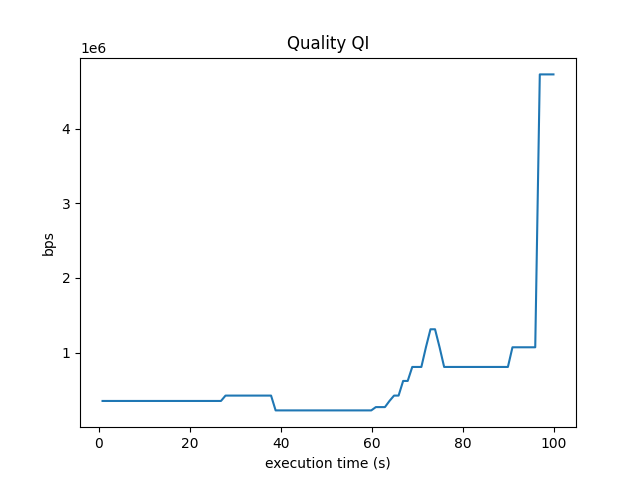
\includegraphics[width=\linewidth]{0.35 - 35 - qual.png}
		\caption{Gráfico de qualidade: $w$ = 0.35, $B_{min}$ = 35}
		\label{fig:1}
	\end{figure}
	\begin{figure}
		\centering
		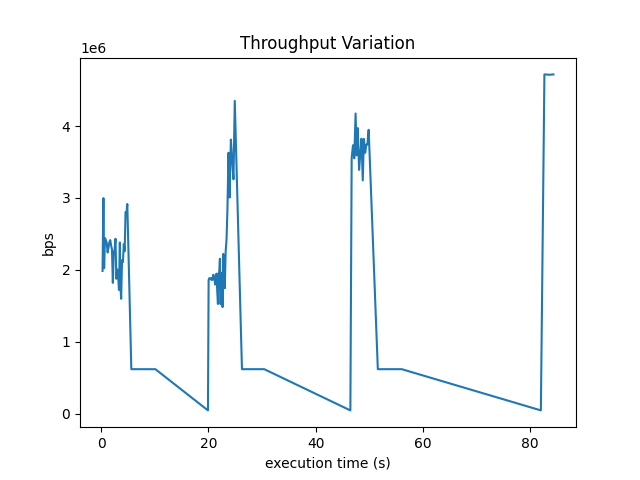
\includegraphics[width=\linewidth]{0.358 -35 -throughput.png}
		\caption{Gráfico de troughput: $w$ = 0.35, $B_{min}$ = 35}
		\label{fig:2}
	\end{figure}
	\begin{figure}
		\centering
		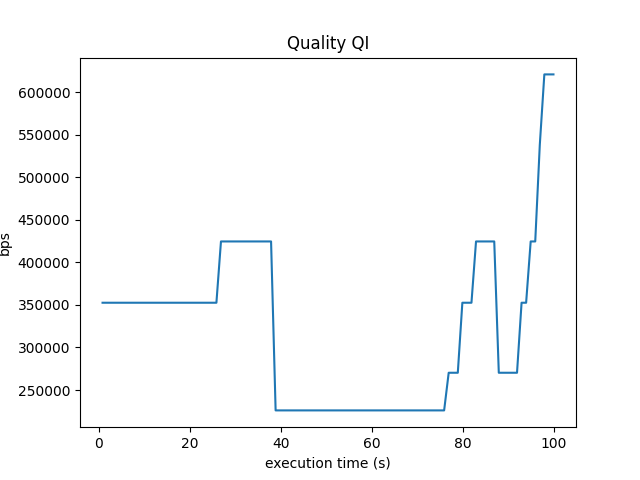
\includegraphics[width=\linewidth]{0.35 - 50 - qual.png}
		\caption{Gráfico de qualidade: $w$ = 0.35, $B_{min}$ = 50}
		\label{fig:3}
	\end{figure}
	\begin{figure}
		\centering
		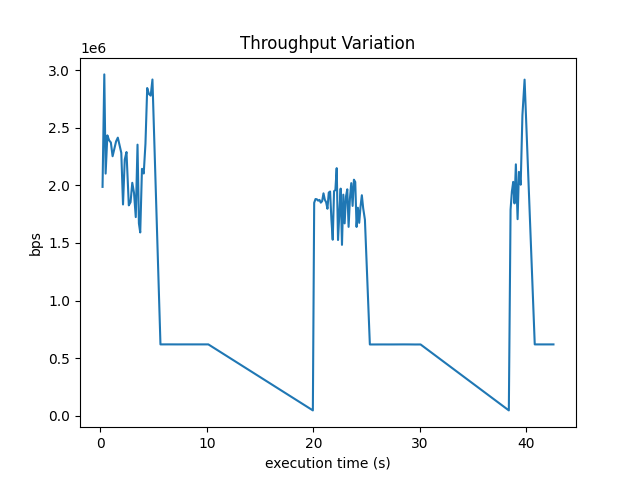
\includegraphics[width=\linewidth]{0.35 - 50 - Throughput .png}
		\caption{Gráfico de troughput: $w$ = 0.35, $B_{min}$ = 50}
		\label{fig:4}
	\end{figure}
	
	\begin{table}[]
		\centering
		\begin{tabular}{c|c|c|c}
			$w$ & $B_{min}$ & Nº(med) de pausas & Tempo de execução  \\
			\hline
			0.3 & 13 & 10 & 233.33 \\
			0.3 & 26 & 4.333 & 160 \\
			\hline
			0.35 &	13&	6.33 & 163.33 \\
			0.35 & 20 &	2&	130 \\
			0.35 & 26 & 2 & 106 \\
			\hline
			0.45 & 13 &	19.33 & 883.33\\
			0.45 & 20 & 9 &	466.66\\
			0.45 & 26 & 1 & 110 \\
			\hline
			0.5 & 13 & 15 & 366.66\\
			0.5 & 20 & 8 & 183.33\\
			0.5 & 26 & 4.33 & 151.66\\
			\hline
			0.6	& 13 & 25 & 1600\\	
			0.6	& 20 & 3 & 126.66 \\
			0.6	& 26 & 3.33 & 266.66 \\
		\end{tabular}
		\caption{Tempo de execução e número de pausas}
		\label{table:1}
	\end{table}
	\begin{table}[]
		\centering
		\begin{tabular}{c|c|c|c}
			$w$ & $B_{min}$  & Tempo de execução & $Q_{max}$ médio \\
			\hline
			0.1 & 13 & 61.66 & 11.3\\
			0.1 & 20 & 66.66 & 11\\
			0.1 & 26 & 61.66 & 12\\
			0.1 & 35 & 56.66 & 11.3 \\
			0.1 & 50 & 45 & 7\\
			\hline
			0.3 & 20 & 80 & 12\\
			0.3 & 35 & 60 & 11\\
			0.3 & 50 & 48.33 & 9.3\\
			\hline
			0.35 & 35 & 81.66 & 13.3\\
			0.35 & 50 & 45 & 12.3\\
			\hline
			0.45 & 35 & 60 & 10\\
			0.45 & 50 & 40 & 9\\
			\hline
			0.5 & 35 & 66.66 & 12\\
			0.5 & 50 & 50 & 10\\
			\hline
			0.6 & 35 & 70 & 10\\
			0.6 & 50 & 46.66 & 12.5\\
		\end{tabular}
		\caption{Tempo de download - Sem pausas}
		\label{table:2}
	\end{table}
	\subsection{Limitador para buffer abaixo de $B_{min}$}
	
	Com a análise de alguns gráficos da sessão anterior, junto à analise do funcionamento do algoritmo, percebemos que este às vezes podia ficar "preso" em qualidades mais altas, estourando o valor de X e Y. Estes, por serem retroalimentados, precisam de um certo tempo para se readequarem ao throughput. Numa rede de alta variação de banda, especialmente em casos de uma rede de baixa velocidade média com picos até 10 a 15 vezes maiores que sua velocidade comum. Isso fazia com que o algoritmo ficasse algum tempo sem conseguir se readequar aos limites da conexão. Para tentar amenizar este problema, foi proposto um limitador para os valores de X[n] e y[n] no caso do tamanho do buffer ser inferior a $B_{min}$. O limite imposto é de até 4 vezes o valor do throughput real.
	
	Como resultado da modificação, foi possível observar uma imediata queda na quantidade de pausas na execução do vídeo. Enquanto as execuções dos diversos testes anteriores retornaram uma quantidade média de pausas de 46\% de acordo com os parâmetros, os mesmos parâmetros retornaram uma média de 23\% nos testes refeitos. A quantidade de pausas deixou de variar de até 25 pausas na execução, como visto na figura \ref{fig:6}, para um máximo de 4, como visto em \ref{fig:5} . Como desvantagem para esta versão do algortimo, nas redes variáveis usadas para teste, há uma menor tendência a atingir os valores altos de pico previamente atingidos.
	
	Também foram realizados testes para verificação do funcionamento do algoritmo em redes estáveis. Foi percebida uma latência para que este se ajuste a qualidade real da rede, mas esta é relativa ao tamanho de $B_{min}$ e não costuma causar grandes prejuízos,como evidenciado nas imagens \ref{fig:7}, \ref{fig:8}, \ref{fig:9} e \ref{fig:10}.
	
	\begin{figure}
		\centering
		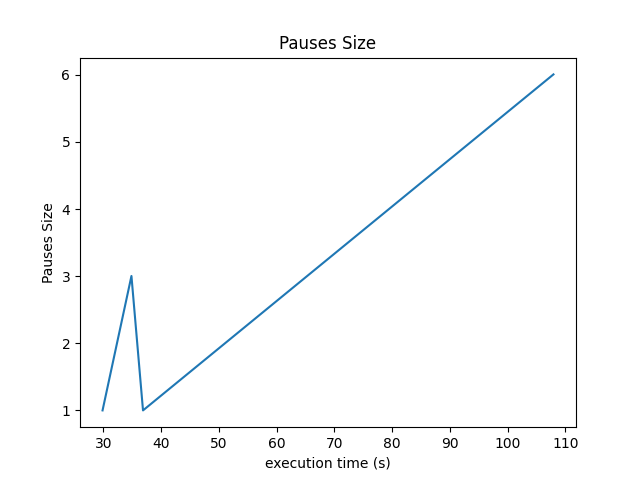
\includegraphics[width=\linewidth]{playback_pauses.png}
		\caption{Pior caso de pausas na execução - Com limitador}
		\label{fig:5}
	\end{figure}
	\begin{figure}
		\centering
		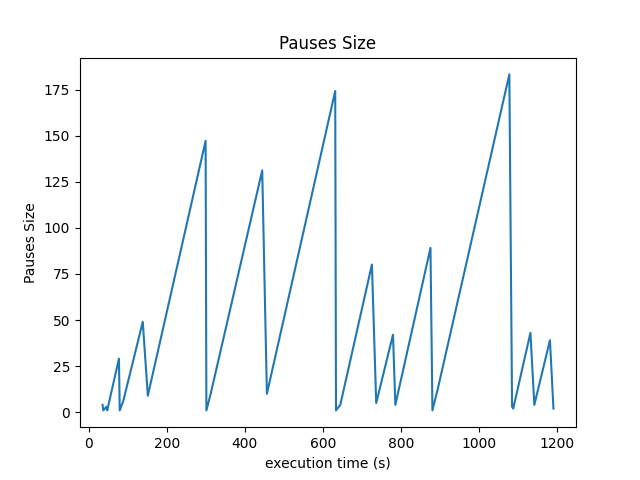
\includegraphics[width=\linewidth]{playback_pauses_25.png}
		\caption{Pior caso de pausas na execução - PANDA}
		\label{fig:6}
	\end{figure}
	\begin{figure}
		\centering
		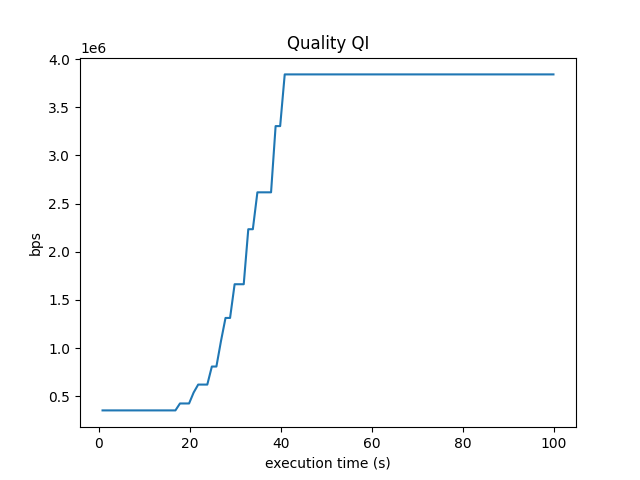
\includegraphics[width=\linewidth]{playback_quality_qi.png}
		\caption{Teste de Qualidade em Baixa Restrição - Buffer mínimo em 13}
		\label{fig:7}
	\end{figure}
	\begin{figure}
		\centering
		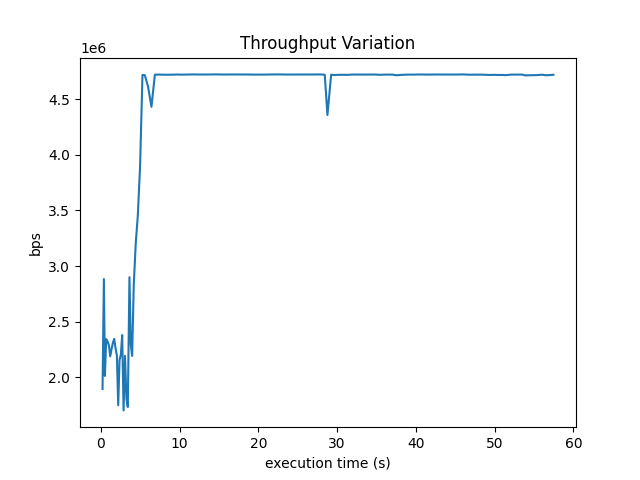
\includegraphics[width=\linewidth]{throughput.png}
		\caption{Teste de Troughput em Baixa Restrição - Buffer mínimo em 13}
		\label{fig:8}
	\end{figure}
	\begin{figure}
		\centering
		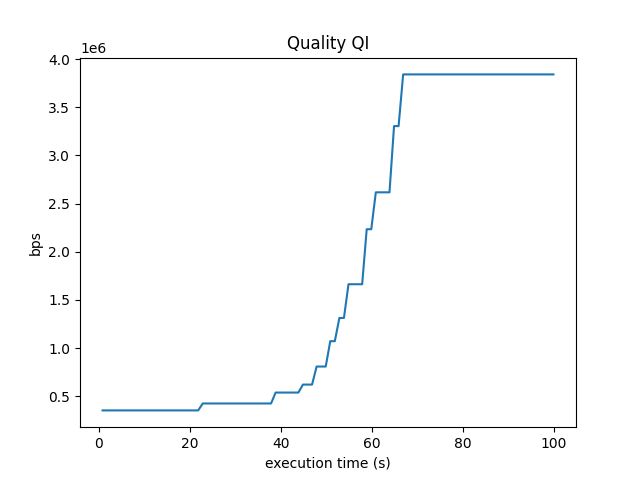
\includegraphics[width=\linewidth]{playback_quality_qi35.png}
		\caption{Teste de Qualidade em Baixa Restrição - Buffer mínimo em 35}
		\label{fig:9}
	\end{figure}
	
	\begin{figure}
		\centering
		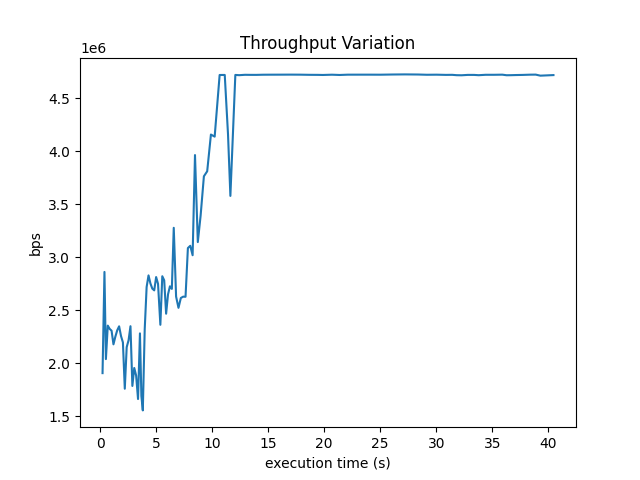
\includegraphics[width=\linewidth]{throughput35.png}
		\caption{Teste de Troughput em Baixa Restrição - Buffer mínimo em 35}
		\label{fig:10}
	\end{figure}
	\section{Conclusões}
	Considerando os resultados apresentados na sessão anterior, conclui-se que o algoritmo proposto satisfaz as condições esperadas de aproveitamento de banda e continuidade de reprodução, apesar de ser necessária uma escolha apropriada de parâmetros, especialmente com relação ao tamanho mínimo do buffer e o incremento de prova do bitrate, uma vez que atuam diretamente na qualidade obtida e na estabilidade da execução. 
	
	O algoritmo mostrou uma clara preferência por valores maiores de tamanho mínimos do buffer quando pareado com valores maiores de $w$. A correlação entre o aumento do valores necessários para a estabilidade pode ser explicada pelo fato de que maiores valores de $w$ aumentam a instabilidade do algoritmo, fazendo com que este tenha facilidade maior de aumentar/diminuir os valores de bitrate a serem requisitados, e necessitando, assim, de um buffer maior para suportar estas mudanças. 
	
	A mudançam proposta para o algoritmo na tentativa de reduzir o número de pausas foi bem sucedida, reduzindo na metade o número de execuções com pausas encontrados nos mesmos testes executados previamente, ao mesmo tempo que reduziu o número máximo de pausas em uma execução de 25 para 4 pausas. 
	
	Quanto à execução do algoritmo em redes com menor alternância de valores de throughput, o algoritmo funcionou satisfatoriamente, apesar de ter uma certa latência causada pelo tempo necessário para carregar o buffer no momento inicial da execução. 
	
	No geral, o trabalho foi um excelente exercício sobre a complexidade de algoritmos que estão ao nosso redor e acabam passando despercebidos. O uso de streaming de vídeo, algo que faz parte do dia a dia, como exercício da matéria permitiu que tivéssemos maior entendimento do funcionamento de protocolos como o DASH e como este lida com a questão do transporte contínuo de dados. A implementação de um algoritmo ABR permitiu ainda exercitar formas de lidar com situações mais reais, com variações constantes no tempo de entrega de pacotes e na forma com que a variação de largura de banda pode tornar a experiência de streaming extremamente desagradável, se não impossível.
	
	{\small
		\bibliographystyle{ieee}
		\bibliography{egbib}
	}
	
\end{document}
